\section{Explanation}

The diagrams below show the total momentum of the system combined with the components of the individual momenta for the Inelastic 2 trial. It shows that the system momentum stays constant despite the components changes.

\begin{figure}[H]
    \centering
    \begin{subfigure}{0.48\textwidth}
        \centering
        % Inelastic 2 initial: p1 = (1.610,-0.170), p2 = (-0.850,-0.500), resultant = (0.760,-0.670)
        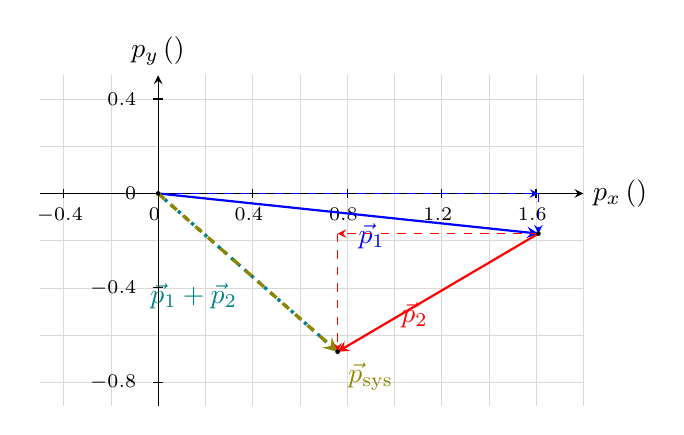
\begin{tikzpicture}[scale=3,>=stealth]
            % grid (fine) + major tick labels with units
            \draw[step=0.2, gray!30, very thin] (-0.5,-0.9) grid (1.8,0.5);
            % major ticks and labels (x)
            \foreach \x in {-0.4,0,0.4,0.8,1.2,1.6}{
                \draw (\x,0.02) -- (\x,-0.02) node[below,font=\scriptsize] {\(\x\ \ns\)};
            }
            % major ticks and labels (y)
            \foreach \y in {-0.8,-0.4,0,0.4}{
                \draw (0.02,\y) -- (-0.02,\y) node[left,font=\scriptsize] {\(\y\ \ns\)};
            }
            % axes with units
            \draw[->, black] (-0.5,0) -- (1.8,0) node[right] {$p_x$\,(\ns)};
            \draw[->, black] (0,-0.9) -- (0,0.5) node[above] {$p_y$\,(\ns)};
            % p1 vector and components (initial)
            \draw[->, blue, thick] (0,0) -- (1.61,-0.17) node[midway, below right] {$\vec p_1$};
            \draw[->, blue, dashed] (0,0) -- (1.61,0);
            \draw[->, blue, dashed] (1.61,0) -- (1.61,-0.17);
            % p2 vector and components (drawn from tip of p1)
            \draw[->, red, thick] (1.61,-0.17) -- (0.76,-0.67) node[midway, below left] {$\vec p_2$};
            \draw[->, red, dashed] (1.61,-0.17) -- (0.76,-0.17);
            \draw[->, red, dashed] (0.76,-0.17) -- (0.76,-0.67);
            % tip-to-tail resultant and system momentum
            \draw[dotted, teal, very thick] (0,0) -- (0.76,-0.67) node[midway, below left] {$\vec p_1+\vec p_2$};
            \draw[->, olive, dashed, very thick] (0,0) -- (0.76,-0.67) node[below right] {$\vec p_{\mathrm{sys}}$};
            % markers
            \fill (0,0) circle (0.01);
            \fill (1.61,-0.17) circle (0.01);
            \fill (0.76,-0.67) circle (0.01);
        \end{tikzpicture}
        \caption{Initial momenta and components (Inelastic 2)}
    \end{subfigure}%
    \hfill
    \begin{subfigure}{0.48\textwidth}
        \centering
        % Inelastic 2 final: p1' = (0.620,-0.810), p2' = (0.140,0.140), resultant = (0.760,-0.670)
        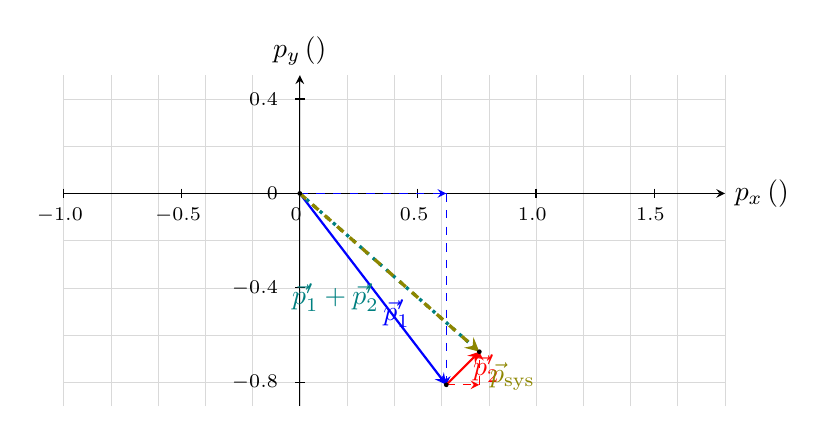
\begin{tikzpicture}[scale=3,>=stealth]
            % grid (fine) + major tick labels with units
            \draw[step=0.2, gray!30, very thin] (-1.0,-0.9) grid (1.8,0.5);
            % major ticks and labels (x)
            \foreach \x in {-1.0,-0.5,0,0.5,1.0,1.5}{
                \draw (\x,0.02) -- (\x,-0.02) node[below,font=\scriptsize] {\(\x\ \ns\)};
            }
            % major ticks and labels (y)
            \foreach \y in {-0.8,-0.4,0,0.4}{
                \draw (0.02,\y) -- (-0.02,\y) node[left,font=\scriptsize] {\(\y\ \ns\)};
            }
            % axes with units
            \draw[->, black] (-1.0,0) -- (1.8,0) node[right] {$p_x$\,(\ns)};
            \draw[->, black] (0,-0.9) -- (0,0.5) node[above] {$p_y$\,(\ns)};
            % p1' vector and components (final)
            \draw[->, blue, thick] (0,0) -- (0.62,-0.81) node[midway, below right] {$\vec p_1'$};
            \draw[->, blue, dashed] (0,0) -- (0.62,0);
            \draw[->, blue, dashed] (0.62,0) -- (0.62,-0.81);
            % p2' vector and components (from tip of p1')
            \draw[->, red, thick] (0.62,-0.81) -- (0.76,-0.67) node[midway, right] {$\vec p_2'$};
            \draw[->, red, dashed] (0.62,-0.81) -- (0.76,-0.81);
            \draw[->, red, dashed] (0.76,-0.81) -- (0.76,-0.67);
            % tip-to-tail resultant and system momentum
            \draw[dotted, teal, very thick] (0,0) -- (0.76,-0.67) node[midway, below left] {$\vec p_1'+\vec p_2'$};
            \draw[->, olive, dashed, very thick] (0,0) -- (0.76,-0.67) node[below right] {$\vec p_{\mathrm{sys}}$};
            % markers
            \fill (0,0) circle (0.01);
            \fill (0.62,-0.81) circle (0.01);
            \fill (0.76,-0.67) circle (0.01);
        \end{tikzpicture}
        \caption{Final momenta and components (Inelastic 2)}
    \end{subfigure}
    \caption{Tip-to-tail addition of components of momenta}
    \label{fig:momentum-tip-to-tail-inelastic2}
\end{figure}

\begin{align*}
\text{Initial (Inelastic 2):}\quad
&p_{1,i,x}=1.610\ \ns,\quad p_{1,i,y}=-0.170\ \ns,\\
&p_{2,i,x}=-0.850\ \ns,\quad p_{2,i,y}=-0.500\ \ns,\\
&p_{\mathrm{sys},x}=p_{1,i,x}+p_{2,i,x}=0.760\ \ns,\quad
p_{\mathrm{sys},y}=p_{1,i,y}+p_{2,i,y}=-0.670\ \ns
\end{align*}

\begin{align*}
\text{Final (Inelastic 2):}\quad
&p_{1,f,x}=0.620\ \ns,\quad p_{1,f,y}=-0.810\ \ns,\\
&p_{2,f,x}=0.140\ \ns,\quad p_{2,f,y}=0.140\ \ns,\\
&p_{\mathrm{sys},x}=p_{1,f,x}+p_{2,f,x}=0.760\ \ns,\quad
p_{\mathrm{sys},y}=p_{1,f,y}+p_{2,f,y}=-0.670\ \ns
\end{align*}

In both the initial and final states, the system momentum is the same. Despite the x and y components being different, they still add up to the same point in space (0.760 \ns~right and 0.670 \ns~down). This can be explained using Newton's third law of motion:

\begin{center}
For every action, there is an equal and opposite reaction.
\end{center}

When you push on an object, it pushes back on you with the same amount of force. If you were ice skating with a friend of the same weight and pushed on them, you would move in opposite directions at the same speed. You would have equal, but opposite momenta.

When stationary, your total momentum is zero. After pushing, your total momentum is still zero because they cancel each other out. In a closed system, you can only deliver impulses to each other. The total momentum cannot change because any change in your momentum would be balanced by an equal and opposite change in your friend's momentum.